\documentclass[aspectratio=169,10pt]{beamer}

\usetheme{Madrid}
\usecolortheme{seahorse}
\usepackage{amsmath,amssymb,amsfonts,mathtools}
\usepackage{listings}
\usepackage{color}
\usepackage{xcolor}
\usepackage{fancybox}
\usepackage{tikz}
\usepackage{graphicx}

\graphicspath{{figures/}}

% Code listings configuration
\lstset{
    basicstyle=\ttfamily\scriptsize,
    numbers=left,
    numberstyle=\tiny\color{gray},
    frame=single,
    language=Python,
    breaklines=true,
    commentstyle=\color{green!50!black}\itshape,
    keywordstyle=\color{blue},
    stringstyle=\color{red},
    stepnumber=1,
    numbersep=8pt,
    escapechar=\#,
}

% Custom colors
\definecolor{darkblue}{rgb}{0, 0, 0.55}
\definecolor{darkgreen}{rgb}{0, 0.55, 0}

% Footer
\setbeamertemplate{footline}[frame number]

\title{Chapter 9: Lower Semicontinuous Convex Functions}
\subtitle{Convex Analysis and Monotone Operator Theory in Hilbert Spaces}
\author{BC 2e, 2017}
\date{}

\begin{document}

\frame{\titlepage}

% ============================================================================
\section{Introduction and Basic Definitions}
% ============================================================================

\begin{frame}[allowframebreaks]{Chapter Overview}
\textbf{Main Topics:}
\begin{itemize}
    \item \textbf{Lower Semicontinuous Convex Functions ($\Gamma(\mathcal{H})$)}
        \begin{itemize}
            \item Definition and fundamental properties
            \item The lower semicontinuous envelope
        \end{itemize}
    \item \textbf{Proper Lower Semicontinuous Convex Functions ($\Gamma_0(\mathcal{H})$)}
        \begin{itemize}
            \item Definitions and characterization
            \item Central role in this book
        \end{itemize}
    \item \textbf{Affine Minorization}
        \begin{itemize}
            \item Continuous affine minorants
            \item Characterization through subdifferentials
        \end{itemize}
    \item \textbf{Recession Functions}
        \begin{itemize}
            \item Definition and properties
            \item Positively homogeneous structure
        \end{itemize}
    \item \textbf{Construction of Functions in $\Gamma_0(\mathcal{H})$}
        \begin{itemize}
            \item Integral functions
            \item Entropy and divergence examples
        \end{itemize}
\end{itemize}
\end{frame}

\begin{frame}{Lower Semicontinuity Definition}
\textbf{Definition 9.1:} A function $f: \mathcal{H} \to [-\infty, +\infty]$ is \alert{lower semicontinuous} (lsc) if
\[
\forall x \in \mathcal{H}, \quad \liminf_{y \to x} f(y) \geq f(x)
\]

Equivalently:
\begin{itemize}
    \item $\text{lev}_{\leq \xi} f = \{x \in \mathcal{H} : f(x) \leq \xi\}$ is closed for all $\xi \in \mathbb{R}$
    \item The epigraph $\text{epi} f = \{(x, y) \in \mathcal{H} \times \mathbb{R} : y \geq f(x)\}$ is closed
\end{itemize}

\vspace{0.3cm}
\textbf{Key Observation:} Lower semicontinuity allows jump discontinuities \emph{upward} but not \emph{downward}.

\vspace{0.3cm}
\textbf{Notation:} $\Gamma(\mathcal{H})$ denotes the class of all lsc proper convex functions on $\mathcal{H}$.
\end{frame}

\begin{frame}{The Epigraph and Convexity}
\begin{columns}
\begin{column}{0.55\textwidth}
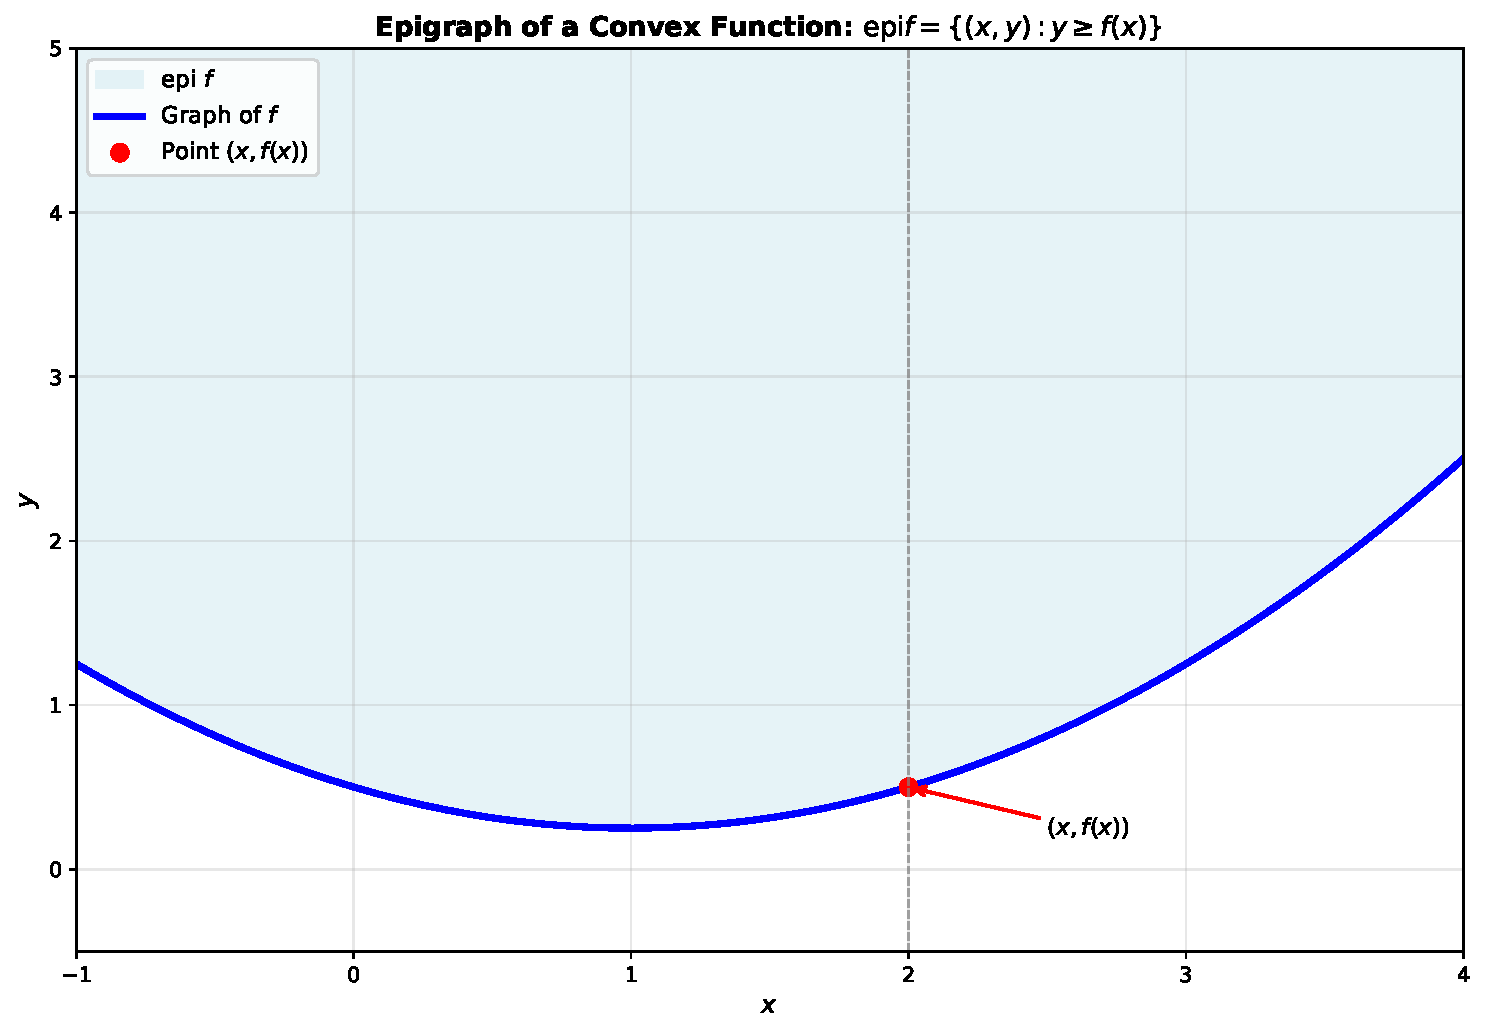
\includegraphics[width=\textwidth]{epigraph.pdf}
\end{column}
\begin{column}{0.45\textwidth}
\textbf{Epigraph Definition:}
\[
\text{epi} f = \{(x, y) \in \mathcal{H} \times \mathbb{R} : y \geq f(x)\}
\]

\vspace{0.2cm}
\textbf{Key Connection:}
\begin{itemize}
    \item $f$ is convex $\iff$ epi $f$ is convex
    \item $f$ is lsc $\iff$ epi $f$ is closed
    \item $f$ is lsc and convex $\iff$ epi $f$ is closed and convex
\end{itemize}

\vspace{0.2cm}
\textbf{Theorem 9.2:} If $f \in \Gamma(\mathcal{H})$, then epi $f$ is a nonempty closed convex subset of $\mathcal{H} \times \mathbb{R}$.
\end{column}
\end{columns}
\end{frame}

\begin{frame}[fragile]{Numerical Example: Convexity and LSC}
\textbf{Check if a function is in $\Gamma(\mathbb{R})$ --- Key Properties:}

\vspace{0.2cm}
\small
For $f(x) = x^2$, verify convexity and lsc:
\begin{enumerate}
    \item \textbf{Convexity:} For $x_1, x_2 \in \mathbb{R}$ and $\lambda \in [0,1]$:
        \[
        f(\lambda x_1 + (1-\lambda)x_2) \leq \lambda f(x_1) + (1-\lambda)f(x_2)
        \]
    
    \item \textbf{LSC at point $x$:} 
        \[
        \liminf_{y \to x} f(y) \geq f(x)
        \]
    
    \item \textbf{Closed epigraph:} The set $\{(x,y) : y \geq x^2\}$ is closed in $\mathbb{R}^2$
\end{enumerate}

\vspace{0.2cm}
All these conditions are satisfied for $f(x) = x^2$, so $f \in \Gamma_0(\mathbb{R})$.
\end{frame}

% ============================================================================
\section{The Lower Semicontinuous Envelope}
% ============================================================================

\begin{frame}{Definition and Properties of the LSC Envelope}
\textbf{Definition 9.7:} For $f: \mathcal{H} \to [-\infty, +\infty]$, the \alert{lower semicontinuous convex envelope} is
\[
\bar{f} = \sup \{g \in \Gamma(\mathcal{H}) : g \leq f\}
\]

\vspace{0.3cm}
\textbf{Theorem 9.9:} For $f: \mathcal{H} \to [-\infty, +\infty]$:
\[
\text{epi}\bar{f} = \overline{\text{conv}(\text{epi} f)}
\]

That is, the epigraph of $\bar{f}$ is the closed convex hull of the epigraph of $f$.

\vspace{0.3cm}
\textbf{Theorem 9.10:} If $f$ is already convex, then $\bar{f} = f$.

\vspace{0.3cm}
\textbf{Corollary 9.11:} If $f$ is convex and $\text{lev}_{<0} f \neq \emptyset$, then
\[
\text{lev}_{<0} f \subset \text{lev}_{<0} \bar{f} \subset \text{lev}_{\leq 0} f
\]
\end{frame}

\begin{frame}{LSC Envelope Visualization}
\begin{columns}
\begin{column}{0.55\textwidth}
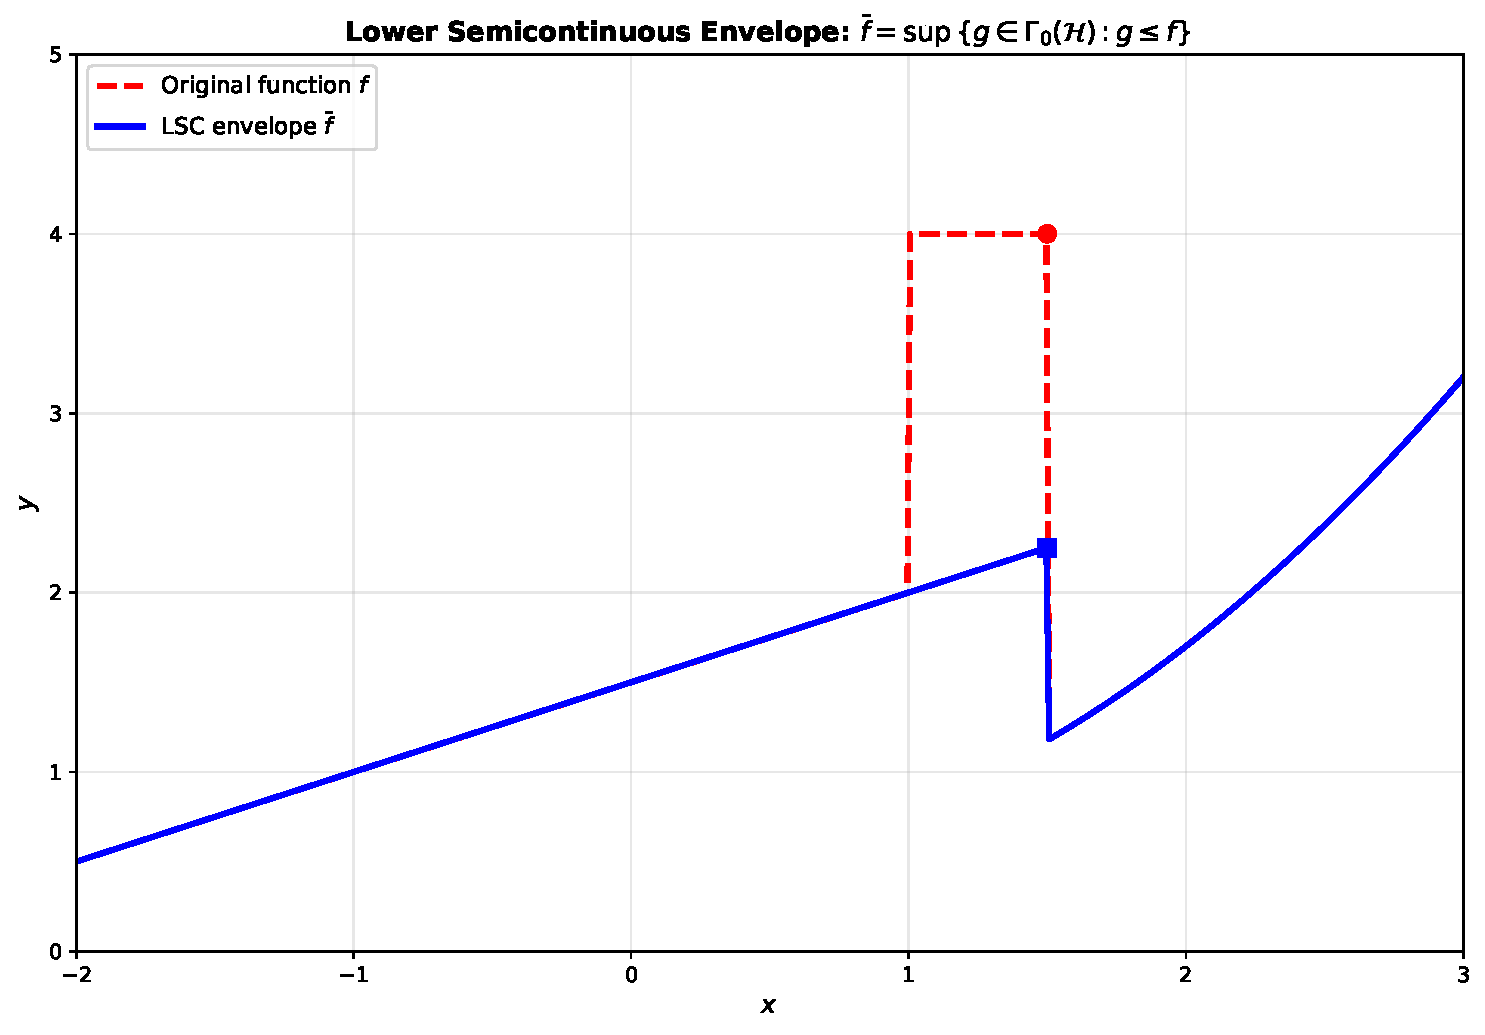
\includegraphics[width=\textwidth]{lsc_envelope.pdf}
\end{column}
\begin{column}{0.45\textwidth}
\textbf{Key Properties:}

\begin{itemize}
    \item $\bar{f}$ is the \emph{largest} lsc convex function below $f$
    \item $\bar{f} \leq f$ everywhere
    \item If $f$ is already lsc and convex, then $\bar{f} = f$
    \item The construction ``fills in'' upward jumps
\end{itemize}

\vspace{0.3cm}
\textbf{Practical Implication:}
\begin{itemize}
    \item Many non-convex or discontinuous functions can be ``corrected'' via their lsc envelope
    \item This provides a canonical way to regularize functions
\end{itemize}
\end{column}
\end{columns}
\end{frame}

% ============================================================================
\section{Proper Lower Semicontinuous Convex Functions}
% ============================================================================

\begin{frame}{Proper Functions}
\textbf{Definition 9.12:} The set of \alert{proper lower semicontinuous convex functions} from $\mathcal{H}$ to $[-\infty, +\infty]$ is denoted $\Gamma_0(\mathcal{H})$.

\vspace{0.3cm}
A function $f$ is proper if:
\begin{enumerate}
    \item $f$ is lower semicontinuous
    \item $f$ is convex
    \item $\text{dom} f \neq \emptyset$ (domain is nonempty)
    \item $f(x) > -\infty$ for all $x$ (never equals $-\infty$)
    \item There exists at least one point where $f(x) < +\infty$
\end{enumerate}

\vspace{0.3cm}
\textbf{Remark:} Nonproper lsc convex functions often have limited usefulness. Proper functions are central to this entire book.

\vspace{0.3cm}
\textbf{Example 9.13:} For families $(e_i)$ and $(\phi_i)$ with appropriate conditions:
\[
f(x) = \sum_{i \in I} \phi_i(\langle x, e_i \rangle) \in \Gamma_0(\mathcal{H})
\]
\end{frame}

\begin{frame}{Basic Properties of $\Gamma_0(\mathcal{H})$}
\textbf{Proposition 9.14:} Let $f \in \Gamma_0(\mathcal{H})$, $x \in \mathcal{H}$, $y \in \text{dom} f$. For $\alpha \in [0,1]$:
\[
\lim_{\alpha \downarrow 0} f(x_\alpha) = f(x)
\]
where $x_\alpha = (1-\alpha)x + \alpha y$.

\vspace{0.3cm}
This is a \emph{directional lower semicontinuity} property.

\vspace{0.3cm}
\textbf{Corollary 9.15:} If $f \in \Gamma_0(\mathbb{R})$, then $f|_{\text{dom} f}$ is continuous.

\vspace{0.3cm}
\textbf{Note:} This fails in general Hilbert spaces! (See Exercise 9.43 with dimension $\mathcal{H} = \mathbb{R}^2$)

\vspace{0.3cm}
\textbf{Fact 9.17:} For $f, g \in \Gamma_0(\mathcal{H})$:
\[
\text{int}(\text{dom} f - \text{dom} g) = \text{core}(\text{dom} f - \text{dom} g)
\]
\end{frame}

% ============================================================================
\section{Affine Minorization}
% ============================================================================

\begin{frame}{Affine Minorization Theorem}
\textbf{Theorem 9.20:} Let $f \in \Gamma_0(\mathcal{H})$. Then $f$ possesses a continuous affine minorant. More precisely,
\[
\exists p \in \text{dom} f, \exists u \in \mathcal{H}, \quad \forall y \in \mathcal{H}: \quad \langle y - p \mid u \rangle + f(p) \leq f(y)
\]

\vspace{0.3cm}
\textbf{Proof Idea:} 
\begin{itemize}
    \item Choose $x \in \text{dom} f$ and $\xi \in (-\infty, f(x))$
    \item Apply the separation theorem for closed convex sets
    \item The separating hyperplane becomes the affine minorant
\end{itemize}

\vspace{0.3cm}
\textbf{Corollary 9.21:} Let $f \in \Gamma_0(\mathcal{H})$. Then $f$ is bounded below on every nonempty bounded subset of $\mathcal{H}$.

\vspace{0.3cm}
\textbf{Example 9.22:} A discontinuous linear functional has no continuous affine minorant!
\end{frame}

\begin{frame}{Supporting Affine Functions}
\textbf{Proposition 9.18:} Let $f \in \Gamma_0(\mathcal{H})$, $(x, \xi) \in \mathcal{H} \times \mathbb{R}$, $(p, \pi) \in \mathcal{H} \times \mathbb{R}$. Then $(p, \pi) = \mathcal{P}_{\text{epi} f}(x, \xi)$ iff:
\[
\max\{\xi, f(p)\} \leq \pi \quad \text{and}
\]
\[
\forall y \in \text{dom} f: \quad \langle y - p \mid x - p \rangle + (f(y) - f(p))(f(p) - \xi) \leq 0
\]

\vspace{0.3cm}
\textbf{Proposition 9.19:} For $f \in \Gamma_0(\mathcal{H})$, $x \in \text{dom} f$, $\xi \in ]-\infty, f(x)[$ and $(p, \pi) \in \mathcal{H} \times \mathbb{R}$:
\[
(p, \pi) = \mathcal{P}_{\text{epi} f}(x, \xi) \iff \xi < f(p) = \pi \text{ and } \forall y \in \text{dom} f: \langle y - p \mid x - p \rangle \leq (f(y) - f(p))(f(p) - \xi)
\]
\end{frame}

\begin{frame}{Affine Minorization Visualization}
\begin{columns}
\begin{column}{0.55\textwidth}
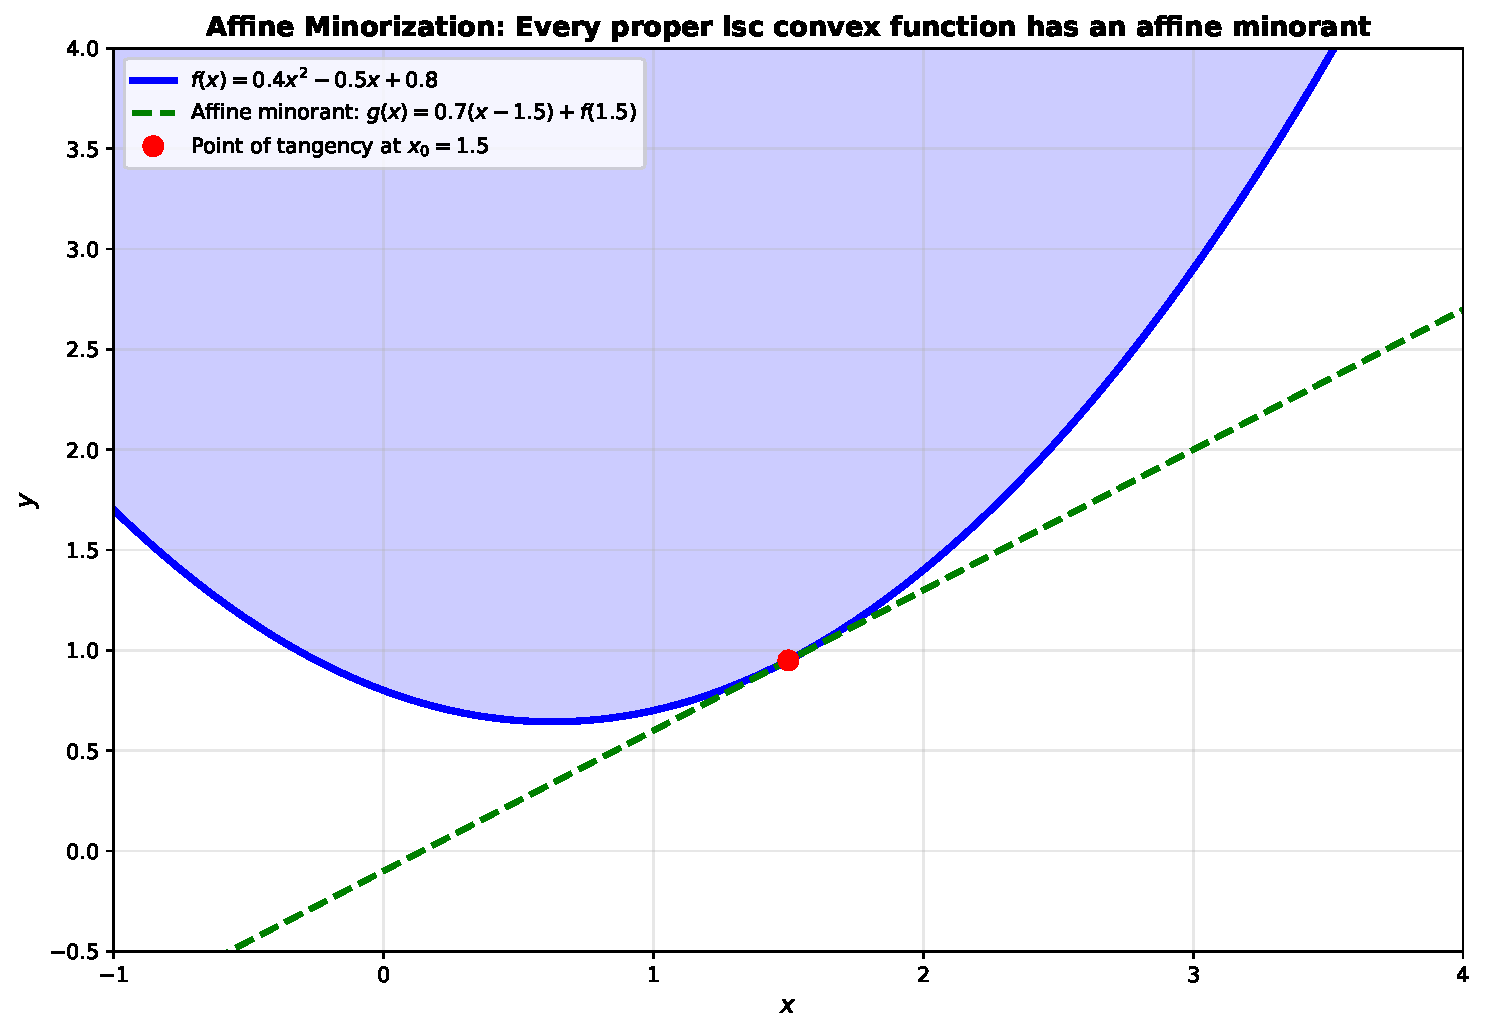
\includegraphics[width=\textwidth]{affine_minorant.pdf}
\end{column}
\begin{column}{0.45\textwidth}
\textbf{Key Points:}

\begin{itemize}
    \item Every proper lsc convex function has supporting hyperplanes
    \item These hyperplanes are continuous affine functions
    \item They provide lower bounds (minorants)
    \item Fundamental for subdifferential calculus
\end{itemize}

\vspace{0.3cm}
\textbf{Application - Subdifferential:}

\medskip
Theorem 9.23: If $x$ is in the interior of dom $f$, then
\[
\exists u \in \mathcal{H}, \exists \eta \in \mathbb{R}: \quad f(y) \geq \langle y - x \mid u \rangle + f(x)
\]

This is the subdifferential condition!
\end{column}
\end{columns}
\end{frame}

\begin{frame}{Jensen's Inequality}
\textbf{Proposition 9.24 (Jensen's Inequality):} Let $(\Omega, \mathcal{F}, \mu)$ be a measure space, $\phi \in \Gamma_0(\mathbb{R})$, and $x: \Omega \to \mathbb{R}$ measurable with $\mu(\Omega)^{-1} \int_\Omega x(\omega)\mu(d\omega) \in \text{dom} \phi$. Then
\[
\phi\left(\frac{1}{\mu(\Omega)} \int_\Omega x(\omega) \mu(d\omega)\right) \leq \frac{1}{\mu(\Omega)} \int_\Omega \phi(x(\omega)) \mu(d\omega)
\]

\vspace{0.3cm}
\textbf{Proof:} Use affine minorization to find $\psi(y) = cy + d$ with $\phi(y) \geq \psi(y)$. Then integrate.

\vspace{0.3cm}
\textbf{Example 9.25:} If $p < q$ and $X$ is a random variable with $\mathbb{E}[|X|^p] < \infty$:
\[
\mathbb{E}[|X|^p]^{1/p} \leq \mathbb{E}[|X|^q]^{1/q}
\]
This follows from Jensen with $\phi(x) = |x|^q / p^{q/p}$.
\end{frame}

% ============================================================================
\section{Recession Functions}
% ============================================================================

\begin{frame}{Definition of Recession Functions}
\textbf{Proposition 9.27:} Let $f: \mathcal{H} \to [-\infty, +\infty]$ be proper and convex, $x \in \text{dom} f$, $y \in \mathcal{H}$. Set
\[
\phi: \mathbb{R}_+ \to [-\infty, +\infty], \quad \alpha \mapsto \frac{f(x + \alpha y) - f(x)}{\alpha}
\]
Then $\phi$ is increasing.

\vspace{0.3cm}
\textbf{Definition 9.28:} For $f: \mathcal{H} \to [-\infty, +\infty]$ proper and convex, the \alert{recession function} at $y \in \mathcal{H}$ is
\[
(\text{rec} f)(y) = \sup_{x \in \text{dom} f} \left(\frac{f(x + y) - f(x)}{1}\right)
\]

Actually, by Proposition 9.27:
\[
(\text{rec} f)(y) = \lim_{\alpha \to \infty} \frac{f(x + \alpha y) - f(x)}{\alpha}
\]
for any fixed $x \in \text{dom} f$.
\end{frame}

\begin{frame}{Properties of Recession Functions}
\textbf{Proposition 9.30:} Let $f \in \Gamma_0(\mathcal{H})$, $x \in \text{dom} f$, $y \in \mathcal{H}$. Then:
\begin{enumerate}
    \item $\text{rec} f \in \Gamma_0(\mathcal{H})$
    \item $(\text{rec} f)(y) = \lim_{\alpha \to +\infty} \frac{f(x + \alpha y) - f(x)}{\alpha}$ (independent of $x$)
    \item $(\text{rec} f)(y) = \lim_{\alpha \to +\infty} f(x + \alpha y) / \alpha$
    \item $(\text{rec} f)(y) = \sup_{\alpha \in \mathbb{R}_+} \frac{f(x + \alpha y) - f(x)}{\alpha}$
    \item If $\inf f(\mathcal{H}) > -\infty$, then $\text{rec} f \geq 0$
    \item If $g \in \Gamma_0(\mathcal{H})$ and $\text{dom} f \cap \text{dom} g \neq \emptyset$, then $\text{rec}(f + g) = \text{rec} f + \text{rec} g$
    \item If $K$ is a Hilbert space, $g \in \Gamma_0(K)$, $L \in \mathcal{B}(\mathcal{H}, K)$, and $\text{ran} L \cap \text{dom} g \neq \emptyset$, then $\text{rec}(g \circ L) = (\text{rec} g) \circ L$
\end{enumerate}
\end{frame}

\begin{frame}{Recession Function Examples and Visualization}
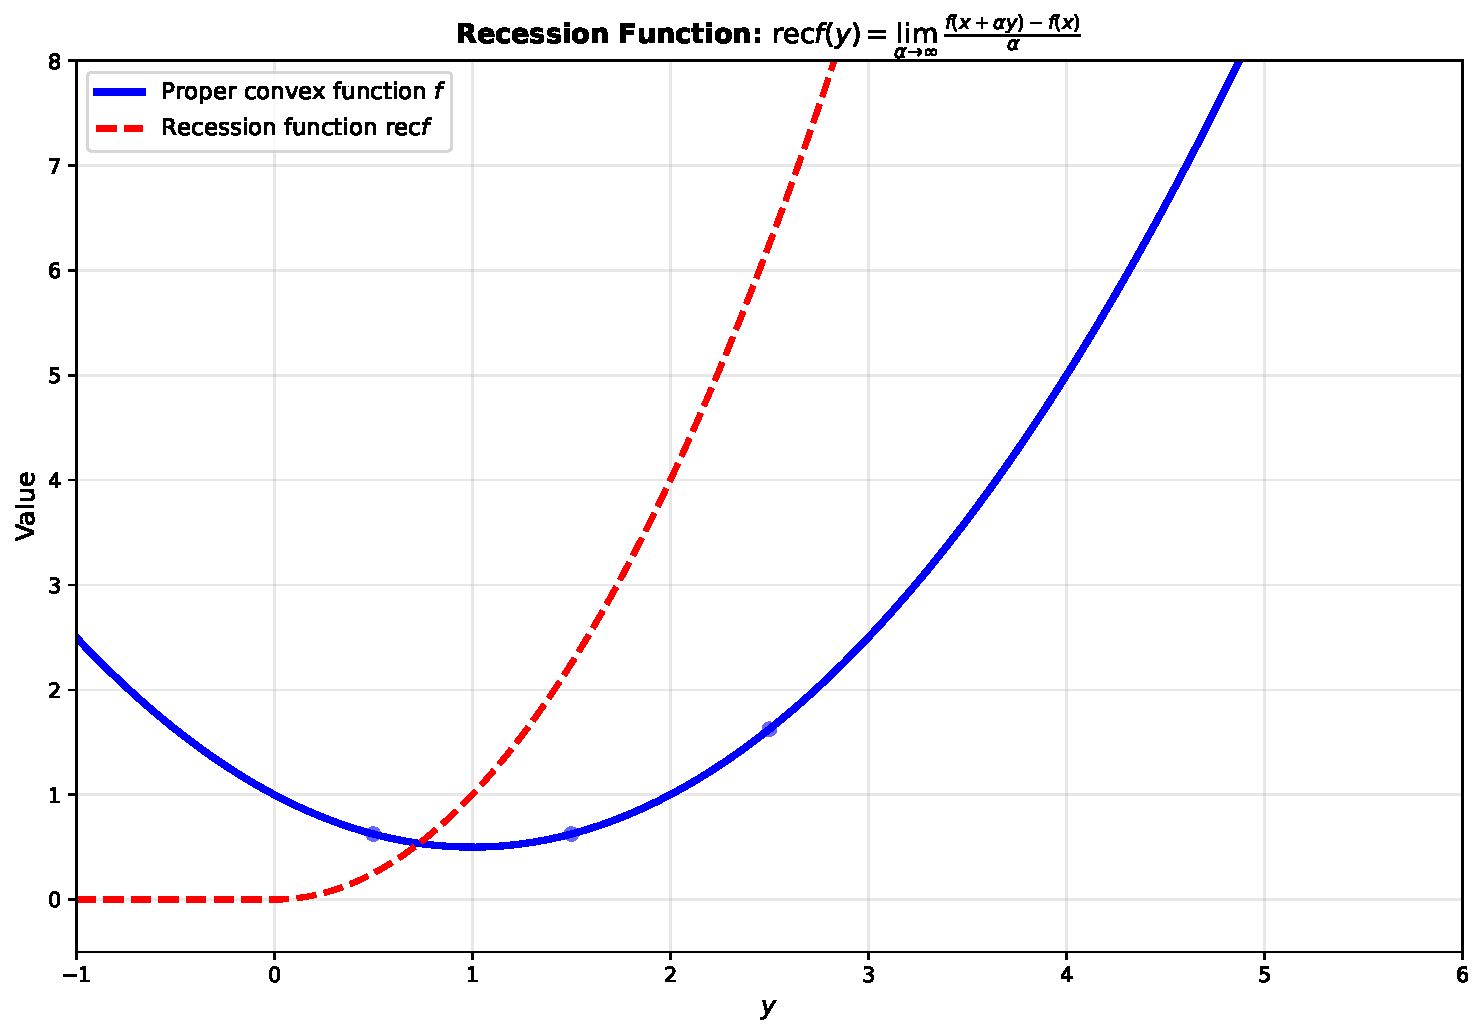
\includegraphics[width=0.7\textwidth]{recession_function.pdf}

\vspace{0.2cm}
\textbf{Example 9.31:} If $f$ is positively homogeneous (i.e., $f(\alpha x) = \alpha f(x)$ for all $\alpha \in \mathbb{R}_+$), then $\text{rec} f = f$.

\vspace{0.2cm}
\textbf{Example 9.32:} For supercoercive $f$ with $\lim_{\|x\| \to \infty} f(x)/\|x\| = +\infty$, we have $\text{rec} f = \iota_{\{0\}}$.
\end{frame}

% ============================================================================
\section{Construction of Functions in Gamma_0}
% ============================================================================

\begin{frame}{Basic Construction: The Closure-Convex Hull Extension}
\textbf{Proposition 9.33:} Let $g: \mathcal{H} \to [-\infty, +\infty]$ be a proper convex function with dom $g$ open and $g$ continuous on dom $g$. Set
\[
f(x) = \begin{cases}
g(x), & \text{if } x \in \text{dom} g \\
\lim_{y \to x} g(y), & \text{if } x \in \text{bdry} \text{dom} g \\
+\infty, & \text{if } x \notin \overline{\text{dom} g}
\end{cases}
\]
Then $f = \bar{g}$ and $f \in \Gamma_0(\mathcal{H})$.

\vspace{0.3cm}
\textbf{Application:} This allows us to take a ``partially defined'' convex function and automatically extend it to a proper lsc function.

\vspace{0.3cm}
\textbf{Example 9.34:} For strictly convex $g: \mathbb{R} \to [-\infty, +\infty]$ on interval $[\alpha, \beta]$:
\[
f(x) = \begin{cases}
g(x), & \text{if } x \in [\alpha, \beta] \\
\lim_{y \uparrow \alpha} g(y), & \text{if } x = \alpha \\
\lim_{y \downarrow \beta} g(y), & \text{if } x = \beta \\
+\infty, & \text{otherwise}
\end{cases}
\in \Gamma_0(\mathbb{R})
\]
\end{frame}

\begin{frame}{Examples of Strictly Convex Functions in $\Gamma_0(\mathbb{R})$}
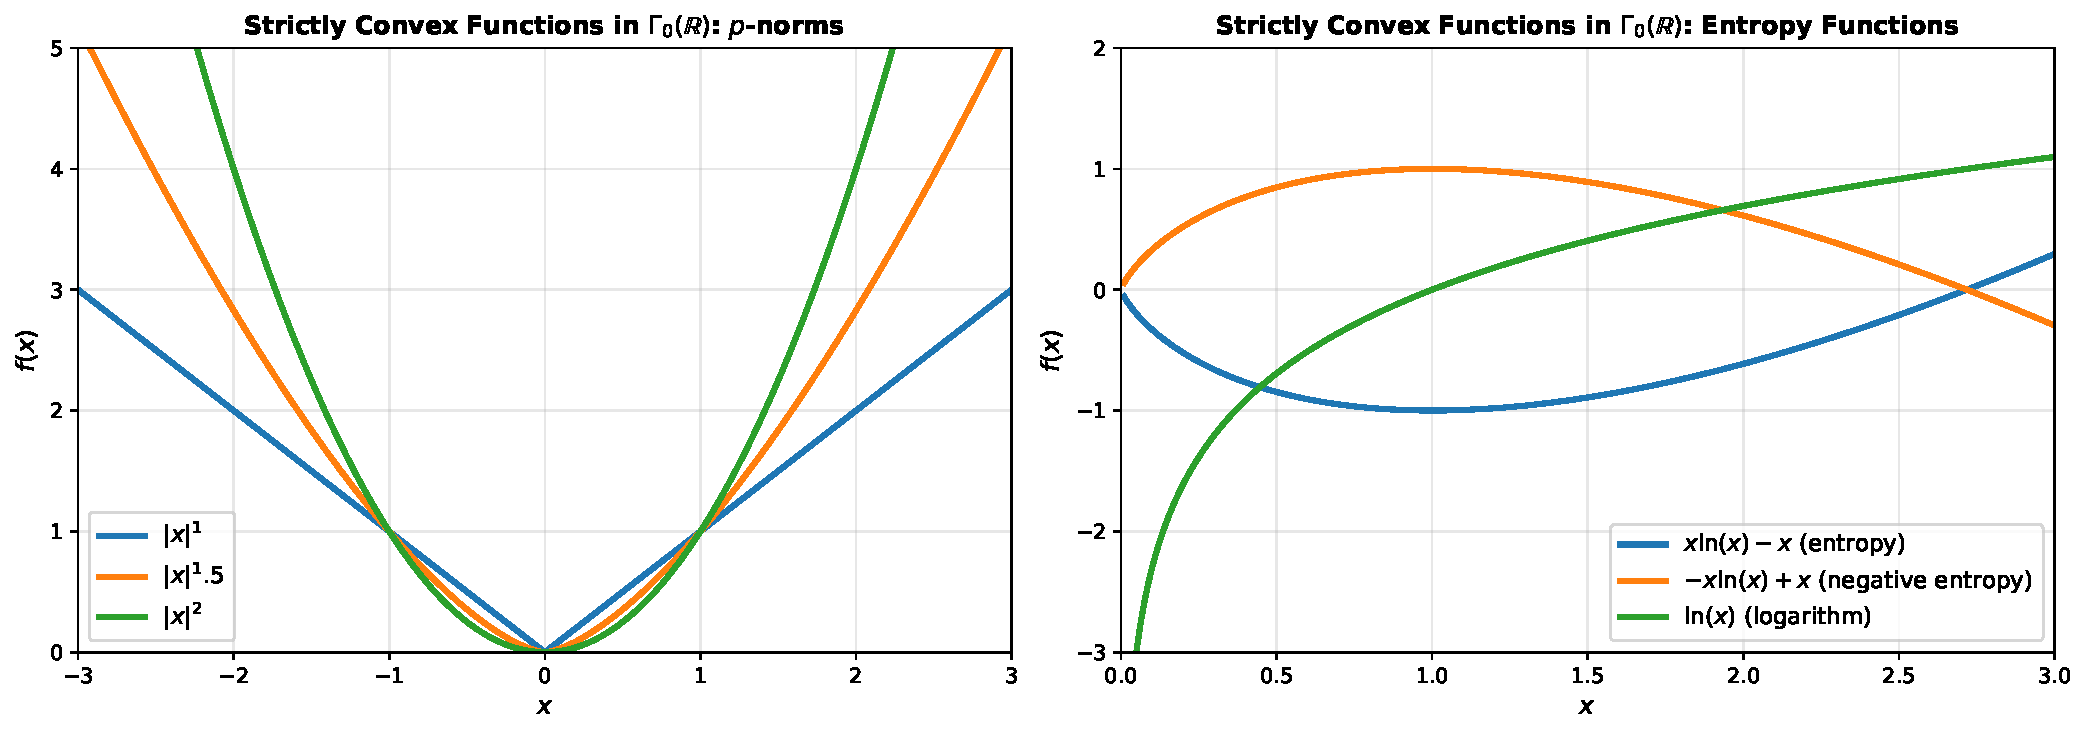
\includegraphics[width=\textwidth]{gamma_zero_functions.pdf}

\textbf{Example 9.36:} The following are all strictly convex in $\Gamma_0(\mathbb{R})$:
\begin{enumerate}
    \item $x \mapsto \exp(x)$
    \item $x \mapsto |x|^p$ for $p \in [1, \infty[$
    \item $x \mapsto 1/x^p$ (for $x > 0$, else $+\infty$) for $p \in [1, \infty[$
    \item $x \mapsto -x^p$ (for $x \geq 0$, else $+\infty$) for $p \in ]0, 1[$
    \item Negative Fermi-Dirac entropy (for $x \in [0,1]$)
    \item $x \mapsto -\ln(x)$ (for $x > 0$, else $+\infty$) — negative Burg entropy
\end{enumerate}
\end{frame}

\begin{frame}{Hölder and Young Inequalities}
\textbf{Proposition 9.38 (Hölder's Inequality):} Let $(\Omega, \mathcal{F}, \mu)$ be a measure space, $p \in [1, \infty[$, and $p^* = p/(p-1)$. For $x \in L^p(\Omega, \mathcal{F}, \mu)$ and $y \in L^{p^*}(\Omega, \mathcal{F}, \mu)$:
\[
\int_\Omega |x(\omega) y(\omega)| \mu(d\omega) \leq \left(\int_\Omega |x(\omega)|^p \mu(d\omega)\right)^{1/p} \left(\int_\Omega |x(\omega)|^{p^*} \mu(d\omega)\right)^{1/p^*}
\]

\vspace{0.3cm}
\textbf{Example 9.39 (Hölder for Sums):} For $x = (\xi_i)_{i \in I}$ and $y = (\eta_i)_{i \in I}$ in $\mathbb{R}^N$:
\[
\sum_{i \in I} |\xi_i \eta_i| \leq \|x\|_p \|y\|_{p^*}
\]
where $\|x\|_p = \left(\sum_{i \in I} |\xi_i|^p\right)^{1/p}$ for $p \in [1, \infty[$, and $\|x\|_\infty = \max_{i \in I} |\xi_i|$.
\end{frame}

\begin{frame}{Integral Functions}
\textbf{Proposition 9.40:} Let $(\Omega, \mathcal{F}, \mu)$ be a measure space, $(\mathcal{H}, \langle \cdot \mid \cdot \rangle_\mathcal{H})$ a separable Hilbert space, and $\varphi \in \Gamma_0(\mathbb{R})$ with:
\begin{enumerate}
    \item $\mu(\Omega) < +\infty$
    \item $\varphi(0) = 0$
\end{enumerate}
Set
\[
f: \mathcal{H} \to [-\infty, +\infty], \quad x \mapsto \begin{cases}
\int_\Omega \varphi(x(\omega)) \mu(d\omega), & \text{if } \varphi \circ x \in L^1((\Omega, \mathcal{F}, \mu); \mathbb{R}) \\
+\infty, & \text{otherwise}
\end{cases}
\]
Then $f \in \Gamma_0(\mathcal{H})$.

\vspace{0.3cm}
\textbf{Intuition:} Integral of proper lsc convex functions yields proper lsc convex functions.
\end{frame}

\begin{frame}{Example: Boltzmann-Shannon Entropy}
\textbf{Example 9.41:} Let $(\Omega, \mathcal{F}, \mathbb{P})$ be a probability space. Using convention $0 \ln(0) = 0$, set
\[
f: L^2(\Omega, \mathcal{F}, \mathbb{P}) \to [-\infty, +\infty], \quad X \mapsto \begin{cases}
\mathbb{E}[X \ln(X) - X], & \text{if } X \geq 0 \text{ a.s.} \\
+\infty, & \text{otherwise}
\end{cases}
\]
Then $f \in \Gamma_0(\mathcal{H})$.

\textbf{Special Cases:}
\begin{enumerate}
    \item \textbf{Entropy of random variable:} $\mathcal{H} = L^2(\Omega, \mathcal{F}, \mathbb{P})$
        \[
        f: X \mapsto \mathbb{E}[X \ln(X) - X], \quad \text{if } X \geq 0 \text{ a.s.}
        \]
    \item \textbf{Discrete entropy:} $\mathcal{H} = \mathbb{R}^N$
        \[
        f: (\xi_k)_{1 \leq k \leq N} \mapsto \sum_{k=1}^N \xi_k \ln(\xi_k) - \xi_k, \quad \text{if } \min_{1 \leq k \leq N} \xi_k \geq 0
        \]
\end{enumerate}
\end{frame}

\begin{frame}{Csiszár $\phi$-Divergence}
\textbf{Example 9.46:} For $\mathcal{H} = \mathbb{R}^N$, $\phi \in \Gamma_0(\mathbb{R})$, the \alert{Csiszár $\phi$-divergence} is a function in $\Gamma_0(\mathcal{H} \oplus \mathcal{H})$ that generalizes:
\begin{itemize}
    \item Kullback-Leibler divergence
    \item Chi-squared divergence
    \item Hellinger distance
    \item And many other divergence measures
\end{itemize}

\vspace{0.3cm}
\textbf{Example 9.48:} The \alert{Kullback-Leibler divergence} 
\[
D_{KL}(p \| q) = \sum_i p_i \ln(p_i / q_i)
\]
is the lsc hull of the KL divergence, and belongs to $\Gamma_0(\mathbb{R}^N \oplus \mathbb{R}^N)$.

\vspace{0.3cm}
\textbf{Remark 9.47:} These divergences appear naturally in:
\begin{itemize}
    \item Information theory and statistics
    \item Machine learning (information bottleneck, clustering)
    \item Variational inference
\end{itemize}
\end{frame}

\begin{frame}{Jensen's Inequality Visualization}

\includegraphics[width=0.8\textwidth]{jensen_inequality.pdf}

The figure illustrates Jensen's inequality: for convex $f$, the function value at the midpoint is below the average of function values at the endpoints.
\end{frame}

% ============================================================================
\section{Perspective Functions and Applications}
% ============================================================================

\begin{frame}{Perspective Functions}
\textbf{Proposition 9.42:} Let $\varphi \in \Gamma_0(\mathcal{H})$. The \alert{perspective function} is
\[
f: \mathbb{R} \times \mathcal{H} \to [-\infty, +\infty], \quad (\xi, x) \mapsto \begin{cases}
\xi \varphi(x/\xi), & \text{if } \xi > 0 \\
+\infty, & \text{otherwise}
\end{cases}
\]
and the \alert{recession of perspective} is
\[
g: \mathbb{R} \times \mathcal{H} \to [-\infty, +\infty], \quad (\xi, x) \mapsto \begin{cases}
\xi \varphi(x/\xi), & \text{if } \xi > 0 \\
(\text{rec} \varphi)(x), & \text{if } \xi = 0 \\
+\infty, & \text{if } \xi < 0
\end{cases}
\]
Then $\bar{f} = g \in \Gamma_0(\mathbb{R} \oplus \mathcal{H})$.

\vspace{0.3cm}
\textbf{Application:} Perspective functions allow scaling with a parameter in convex optimization.
\end{frame}

\begin{frame}{Power-Type Perspective Functions}
\textbf{Example 9.43:} For $p \in [1, \infty[$, the function
\[
g: \mathbb{R} \times \mathcal{H} \to [-\infty, +\infty], \quad (\xi, x) \mapsto \begin{cases}
\|Lx - r\|^p / (\langle x \mid u \rangle - \rho)^{p-1}, & \text{if } \langle x \mid u \rangle > \rho \\
0, & \text{if } \langle x \mid u \rangle = \rho \text{ and } Lx = r \\
+\infty, & \text{otherwise}
\end{cases}
\]
belongs to $\Gamma_0(\mathbb{R} \oplus \mathcal{H})$.

\vspace{0.3cm}
\textbf{Note:} This can be discontinuous at $(0, 0)$, illustrating that $\Gamma_0$ functions can be discontinuous.

\vspace{0.3cm}
\textbf{Generalization (Corollary 9.44):} Similar constructions work for operators $L \in \mathcal{B}(\mathcal{H}, K)$ and affine hyperplanes.
\end{frame}

% ============================================================================
\section{Summary and Connections}
% ============================================================================

\begin{frame}[allowframebreaks]{Key Takeaways}
\textbf{Fundamental Concepts:}

\begin{enumerate}
    \item \textbf{Lower Semicontinuous Functions} allow upward jumps but control behavior via:
        \begin{itemize}
            \item Closed level sets
            \item Closed epigraphs
            \item The lsc envelope construction
        \end{itemize}

    \item \textbf{Proper Functions} are the working class of convex analysis:
        \begin{itemize}
            \item Never take value $-\infty$
            \item Have nonempty domains
            \item Form the class $\Gamma_0(\mathcal{H})$
        \end{itemize}

    \item \textbf{Affine Minorization} is crucial for subdifferential theory:
        \begin{itemize}
            \item Every proper lsc convex function has continuous affine minorants
            \item These form the subdifferential
            \item Jensen's inequality follows from minorization
        \end{itemize}

    \item \textbf{Recession Functions} capture behavior at infinity:
        \begin{itemize}
            \item Control growth rates in all directions
            \item Form a proper lsc convex function themselves
            \item Preserve additivity under summation
        \end{itemize}

    \item \textbf{Construction Methods} show the richness of $\Gamma_0(\mathcal{H})$:
        \begin{itemize}
            \item Integral functions
            \item Entropy and divergence examples
            \item Perspective functions
        \end{itemize}
\end{enumerate}

\framebreak

\textbf{Major Theorems:}

\vspace{0.2cm}
\begin{itemize}
    \item \textbf{Theorem 9.9:} Characterization of lsc envelope via closed convex hull of epigraph
    \item \textbf{Theorem 9.20:} Affine minorization for proper functions
    \item \textbf{Theorem 9.23:} Interior point characterization (subdifferential relation)
    \item \textbf{Proposition 9.24:} Jensen's inequality for measure spaces
    \item \textbf{Proposition 9.30:} Properties and structure of recession functions
    \item \textbf{Proposition 9.40:} Integral functions stay in $\Gamma_0(\mathcal{H})$
\end{itemize}

\vspace{0.3cm}
\textbf{Connection to Later Chapters:}

\begin{itemize}
    \item Chapter 10: Subdifferentials are supported by affine minorants
    \item Chapter 11: Conjugate functions use proper lsc functions
    \item Chapters 12+: Monotone operators and fixed point theory require $\Gamma_0$ structure
\end{itemize}
\end{frame}

\begin{frame}{Historical and Practical Context}
\textbf{Why This Chapter Matters:}

\begin{itemize}
    \item Lower semicontinuous convex functions are the correct framework for optimization
    \item Real-world problems lead naturally to non-smooth, even discontinuous, functions
    \item The lsc envelope allows regularization and approximation
    \item Affine minorization is the foundation of convex analysis
    \item Recession functions characterize behavior at infinity (critical for existence theory)
    \item Entropy and divergence functions are essential in machine learning, statistics, and information theory
\end{itemize}

\vspace{0.4cm}
\textbf{Modern Applications:}
\begin{itemize}
    \item Variational methods in PDEs
    \item Convex optimization algorithms
    \item Machine learning (loss functions, regularizers)
    \item Information theory (entropy, divergences)
    \item Economic equilibrium models
\end{itemize}
\end{frame}

\end{document}
